\documentclass{beamer}
\usepackage[english]{babel}
\usepackage[utf8]{inputenc}
\usepackage[T1]{fontenc}

\usepackage{bm}
%\usepackage{math}
\usepackage{physics}

\usepackage{pgfplots}
% and optionally (as of Pgfplots 1.3):
\pgfplotsset{compat=newest}
\pgfplotsset{plot coordinates/math parser=false}
\newlength\figureheight
\newlength\figurewidth
\usepackage{environ}

\newcommand{\Hilbert}{\mathcal{H}}
\newcommand{\Vector}[1]{\bm{\MakeLowercase{#1}}}
\newcommand{\Operator}[1]{\bm{\MakeUppercase{#1}}}
%%%%%%%%%%
\DeclareMathAlphabet{\mathsfbr}{OT1}{cmss}{m}{n}%for math sans serif (cmss)
\SetMathAlphabet{\mathsfbr}{bold}{OT1}{cmss}{bx}{n}%for math sans serif (cmss)
\DeclareRobustCommand{\msf}[1]{%
  \ifcat\noexpand#1\relax\msfgreek{#1}\else\mathsfbr{#1}\fi%for math sans serif (cmss)
}
\DeclareFontEncoding{LGR}{}{} % or load \usepackage{textgreek}
\DeclareSymbolFont{sfgreek}{LGR}{cmss}{m}{n}
\SetSymbolFont{sfgreek}{bold}{LGR}{cmss}{bx}{n}
\DeclareMathSymbol{\sXi}{\mathalpha}{sfgreek}{`X}
\DeclareMathSymbol{\sUpsilon}{\mathalpha}{sfgreek}{`U}
%%%%%%%%%%

%\usetheme[titlepagelogo=Pictures/logo.png,
%          language=english,
%          bullet=square,
%          color=blue,
%          coding=utf8, % occhio solo a questo, se non funziona usa pure latin1
%          secondsupervisor=false,
%          assistantsupervisor=true,
%         ]{TorinoTh}

\usetheme{Ferrara}

\author[Federico Forzano]{
                        {\scriptsize Supervisor:}\hspace{60mm}{\scriptsize Candidate:}\\
                        Chiar.mo~Prof.~Andrea Conti \hspace{25mm} Federico Forzano\\
                        {\scriptsize Co-Supervisor:}\\
                        Dott.~Ing.~Stefano Guerrini
                        }

\title{On the Design of Quantum Communication Systems with non-Gaussian States}

\date{}

\begin{document}
        
    
    \begin{frame}
    \maketitle
\end{frame}

    % Capitolo 1: Quantum Mechanics Abstract
    %\section{Postulates}
    Like every phisics theory, quantum mechanics is builded from few 
    essential postulates.
    In this section are briefly introduced the six Dirac-Von Newman 
    postulates of Quantum Mechanics \cite{quantumMec_Dirac,quantumMec_Neumann}.
    
    \subsection{First postulate}
    \begin{postulate}[State Representation]
        The state of an isolated quantum system is represented by a complex unitary 
        vector $\ket{\psi}$ in an Hilbert space $\Hilbert$:
        \begin{equation*}
            \ket{\psi} \in \Hilbert
        \end{equation*}
        The space of possible states of the system is called state space and it is a
        separable complex Hilbert space.
        \label{post:1}
    \end{postulate}
    \begin{observation*}
        Differently from the classical physics, in quantum mechanics the concept
        of state of system is introduced. In classical mechanics a system is 
        described by his observables, like position or four-wheeled.
    \end{observation*}
    
    \subsection{Second postulate}
    \begin{postulate}[Observables]
        Every observables of the system is represented by an Hermitian operator $\mathcal{M}$
        acting on the state space:
        \begin{equation*}
            \mathcal{M}:\Hilbert\to\Hilbert
        \end{equation*}
        The outcomes of the measurement can only be one of the eigenvalue of the 
        operator $\mathcal{M}$.
        \label{post:2}
    \end{postulate}
    \begin{observation*}
        The possible outcomes of the measurement are real number because $\mathcal{M}$
        is self-andjoint. 
    \end{observation*}

    \subsection{Third postulate}
    \begin{postulate}[Born's Rule]
        The probability to get the measurement $\lambda_i$ from the observable 
        $\mathcal{M}$ in the system in state $\ket{\psi}$ is:
        \begin{equation*}
            %\mathbb{P}(\lambda_i)=\braket{\psi}{\lambda_i}\braket{\lambda_i}{\psi}
            \mathbb{P}(\lambda_i)=\bra{\psi}\mathcal{P}_i\ket{\psi}
        \end{equation*}
        where $\bra{\psi}$ is the correspondent vector of $\ket{\psi}$ in the 
        dual space of $\Hilbert$ and where $\mathcal{P}_i$ is the projection operator
        of $\lambda_i$ in the correspondent space.
        \label{post:3}
    \end{postulate}

    \subsection{Fourth postulate}
    \begin{postulate}[Wavefunction Collapse]
        The state $\ket{\psi'}$ after measurement of $\lambda_i$ is $\mathcal{P}_i\ket{\psi}$ (with the
        necessary normalization):
        \begin{equation*}
            \ket{\psi'}=\frac{\mathcal{P}_i\ket{\psi}}{\bra{\psi}\mathcal{P}_i\ket{\psi}}.
        \end{equation*}
        \label{post:4}
    \end{postulate}

    \subsection{Fifth postulate}
    \begin{postulate}[Time Evolution]
        The time evolution of an isolated quantum system is given by an unitary operator
        $\mathcal{U}$:
        \begin{equation*}
            \ket{\psi(t)}=\mathcal{U}(t_0,t)\ket{\psi(t_0)}.
        \end{equation*}
        \label{post:5}
    \end{postulate}
    \begin{observation*}[Time dependent Shrodinger Equation]
        From postulate \ref{post:5}, it is possible to obtain the time dependent Shrodinger Equation:
        \begin{equation*}
            i\hbar\partialderivative{}{t}\ket{\psi(t)}=H(t)\ket{\psi(t)}
        \end{equation*}
        where $H(t)$ is the Hemiltonian matrix.
    \end{observation*}

    \subsection{Sixth postulate}
    \begin{postulate}[Composite System]
        The state space $\Hilbert$ of a system composed of $\Hilbert_1$ and $\Hilbert_2$ is given by
        \begin{equation*}
            \Hilbert=\Hilbert_1\otimes\Hilbert_2.
        \end{equation*}
        \label{post:6}
    \end{postulate}

    %\section{Quantized Electromagnetic Field}
    Electromagnetic field is the main means of communication for contemporary
    applications, it is important therefor to give its quantum conception.
    In this section, the representation of quantized electromagnetic field is 
    firstly given, then the Fock's representation of a quantum state is introduced.
            
    \subsection{Classical electromagnetic field}
        In a volume $\mathcal{V}\in\mathbb{R}^3$ classical electromagnetic field is 
        determinated from Maxwell's equations as a superposition of the cavity modes
        (\cite{tesiGuerrini} quoting \cite{quantumRad_Louissel,quantumOptic_Mandel}).
        Electric field is given by the well-known expression:
        \begin{equation}
            \pmb{e}(\pmb{r},t)=-\sum_n p_n (t)\pmb{u}_n (\pmb{r})
            \label{eq:CEF.1}
        \end{equation}
        where
        \begin{equation*}
            \pmb{u}_n (\pmb{r})=\pmb{u}_{n0}\ e^{i\pmb{k}_n \cdot \pmb{r}}
        \end{equation*}
        and $\pmb{u}_{n0}$ is determinated by the initial condition.
        The corresponding magnetic field is determinated by:
        \begin{equation}
            \pmb{h}(\pmb{r},t)=\sum_n q_n (t)\nabla\times\pmb{u}_n (\pmb{r})
            \label{eq:CEF.2}
        \end{equation}
        and
        \begin{equation}
            p_n (t)=\derivative{q_n (t)}{t} .
            \label{eq:CEF.3}
        \end{equation}
        The Hemiltonian associated to the n-th mode is given by
        \begin{equation}
            H_n=\frac{1}{2}[p_n^2(t)+\omega_n^2q_n^2(t)].
            \label{eq:CEF.4}
        \end{equation}
        Equivalently, it is possible to define the complex variable $a_n(t)$ as
        \begin{equation}
            a_n(t)=\frac{\omega_nq_n(t)+ip_n(t)}{\sqrt{2\hbar\omega_n}}
            \label{eq:CEF.5}
        \end{equation}
        and, using \ref{eq:CEF.5} in \ref{eq:CEF.4}, it is possible to obtain the following
        expression of the Hemiltonian:
        \begin{equation}
            H_n=\hbar\omega_n\absolutevalue{a_n(t)}^2.
            \label{eq_CEF.6}
        \end{equation}

    \subsection{Quantized electromagnetic field}
        The quantization of electromagnetic field is obtained replacing the two quantities 
        $p_n(t)$ and $q_n(t)$ with the Hermitian operators 
        $\pmb{P}_n(t),\ \pmb{Q}_n(t):\Hilbert_n\to\Hilbert_n$ and by imposing the following
        commutation conditions (\cite{tesiGuerrini} quoting \cite{quantumRad_Louissel,quantumOptic_Mandel}):
        \begin{equation}
            \commutator{\pmb{Q}_n}{\pmb{P}_m}=i\hbar\delta_{n,m}\pmb{I}
        \end{equation}
        \begin{equation}
            \commutator{\pmb{Q}_n}{\pmb{Q}_m}=0
        \end{equation}
        \begin{equation}
            \commutator{\pmb{P}_n}{\pmb{P}_m}=0.
        \end{equation}
        Defining the annihilation operator $\pmb{A}_n$ as
        \begin{equation}
            \pmb{A}_n(t)=\frac{\omega_n\pmb{Q}_n(t)+i\pmb{P}_n(t)}{\sqrt{2\hbar\omega_n}}
            \label{eq:QEF.1}
        \end{equation} 
        and the adjoint of $\pmb{A}_n$, the creation operator $\pmb{A}_n^\dagger$ as
        \begin{equation}
            \pmb{A}_n(t)=\frac{\omega_n\pmb{Q}_n(t)-i\pmb{P}_n(t)}{\sqrt{2\hbar\omega_n}}
            \label{eq:QEF.2}
        \end{equation}
        it is possible to describe the Hemiltonian of the system as
        \begin{equation}
            H_n=\hbar\omega_n\pmb{A}_n^\dagger\pmb{A}_n.
            \label{eq:QEF.3}
        \end{equation}

    \subsection{Fock states}
        In a single mode cavity, it is possible to define the number operator $\pmb{N}$ as
        \begin{equation}
            \pmb{N}=\pmb{A}^\dagger \pmb{A}.
        \end{equation}
        Single mode Fock states are the eigenvector of $N$, i.e the solution of equation:
        \begin{equation}
            \pmb{N}\ket{n}=n\ket{n}.
        \end{equation}
        The Fock state $\ket{n}$ represents the quantum state with exactly n photons.
        It is important to point out that the set of all Fock states forms an orthonormal basis
        of the Hilbert space $\Hilbert$, so every state $\Xi$ can be expressed as
        \begin{equation}
            \pmb{\Xi} = \sum_{n,m} c_{n,m}\ket{n}\bra{m}
            \label{eq:QEF.4}
        \end{equation}
        with
        \begin{equation*}
            c_{n,m}=\bra{n}\pmb{\Xi}\ket{m}.
        \end{equation*}

        Using the representation in Fock basis, it is possible to characterize different types
        of quantum state of the quantum electromagnetic field. In the following section the 
        states studied are briefly described.
    %\begin{frame}
    \frametitle{Quantum Mechanics Abstract}
    \framesubtitle{Fock states}

    \begin{block}{Fock State}<1->
        The Fock state $\ket{n}$ represents the quantum state with exactly n photons. It is 
        defined as:
        \begin{equation*}
            \pmb{N}\ket{n}=n\ket{n}\ \ with\ \pmb{N}=\pmb{A}^\dagger \pmb{A}
        \end{equation*}
    \end{block}
    \begin{alertblock}{Fock Representation}<2->
        Every quantum state $\pmb{\Xi}$ can be expressed as
        \begin{equation*}
            \pmb{\Xi} = \sum_{n,m} c_{n,m}\ket{n}\bra{m}\ \ with\ c_{n,m}=\bra{n}\pmb{\Xi}\ket{m}
        \end{equation*}
    \end{alertblock}

\end{frame}
    %\begin{frame}{Quantum Mechanics Abstract}{Wigner Function}

\end{frame}
    %\begin{frame}{Quantum Communication System}{Some important states}
    \begin{columns}

        \begin{column}{0.5\textwidth}
            \center{\underline{Coherent state}}
            \begin{equation*}\begin{split}
                &\Operator{A}\ket{\mu}=\mu\ket{\mu}\\
                &\ket{\mu}=\Operator{D}_\mu\ket{0}
            \end{split}\end{equation*}
            \\ \mbox{}
            \center{\underline{Thermal noise state}}
            \begin{equation*}\begin{split}
                &\Operator{\varXi}_{\mathrm{th}}=(1-v)\sum_{n=0}^{\infty}v^n\ket{n}\bra{n}\\
                v=&\frac{\bar{n}}{\bar{n}+1};\ \ \ \ 
                \bar{n}=\left(\exp{\frac{\hbar\omega}{k_B T}}-1\right)^{-1}
            \end{split}\end{equation*}
        \end{column}
        \begin{column}{0.5\textwidth}
            \center{\underline{Squeezed state}}
            \begin{equation*}
                \ket*{\mu,\zeta}=\Operator{D}_\mu\Operator{S}_\zeta\ket{0}
            \end{equation*}
            \\ \mbox{}
            \center{\underline{Photon added states}}\\
            \begin{equation*}
                \Operator{\varXi}^{(k)}=\frac{(\Operator{A}^\dagger)^k\Operator{\varXi}\pmb{A}^k}
                {\tr{(\Operator{A}^\dagger)^k\Operator{\varXi}\Operator{A}^k}}
            \end{equation*}
            \mbox{}
            %\hspace*{30pt}
            \mbox{}
        \end{column}
    \end{columns}

    \ \\ \mbox{} \\ \ \mbox{}
\end{frame}

    \section{Motivation}
    \begin{frame}{Motivation}
    \begin{itemize}
        \item Communications are becoming ever more important and widespread.
        \item Classical physics is only a special case of quantum physics.
        \item The use of quantum non-Gaussian states can significantly improve the performance 
                of a communication system.
    \end{itemize}
\end{frame}
    \begin{frame}{Contents}
        \tableofcontents
    \end{frame}

    % Capitolo 2: Quantum Communication
    \section{Quantum Communication System}
    \begin{frame}{Quantum Communication System}
    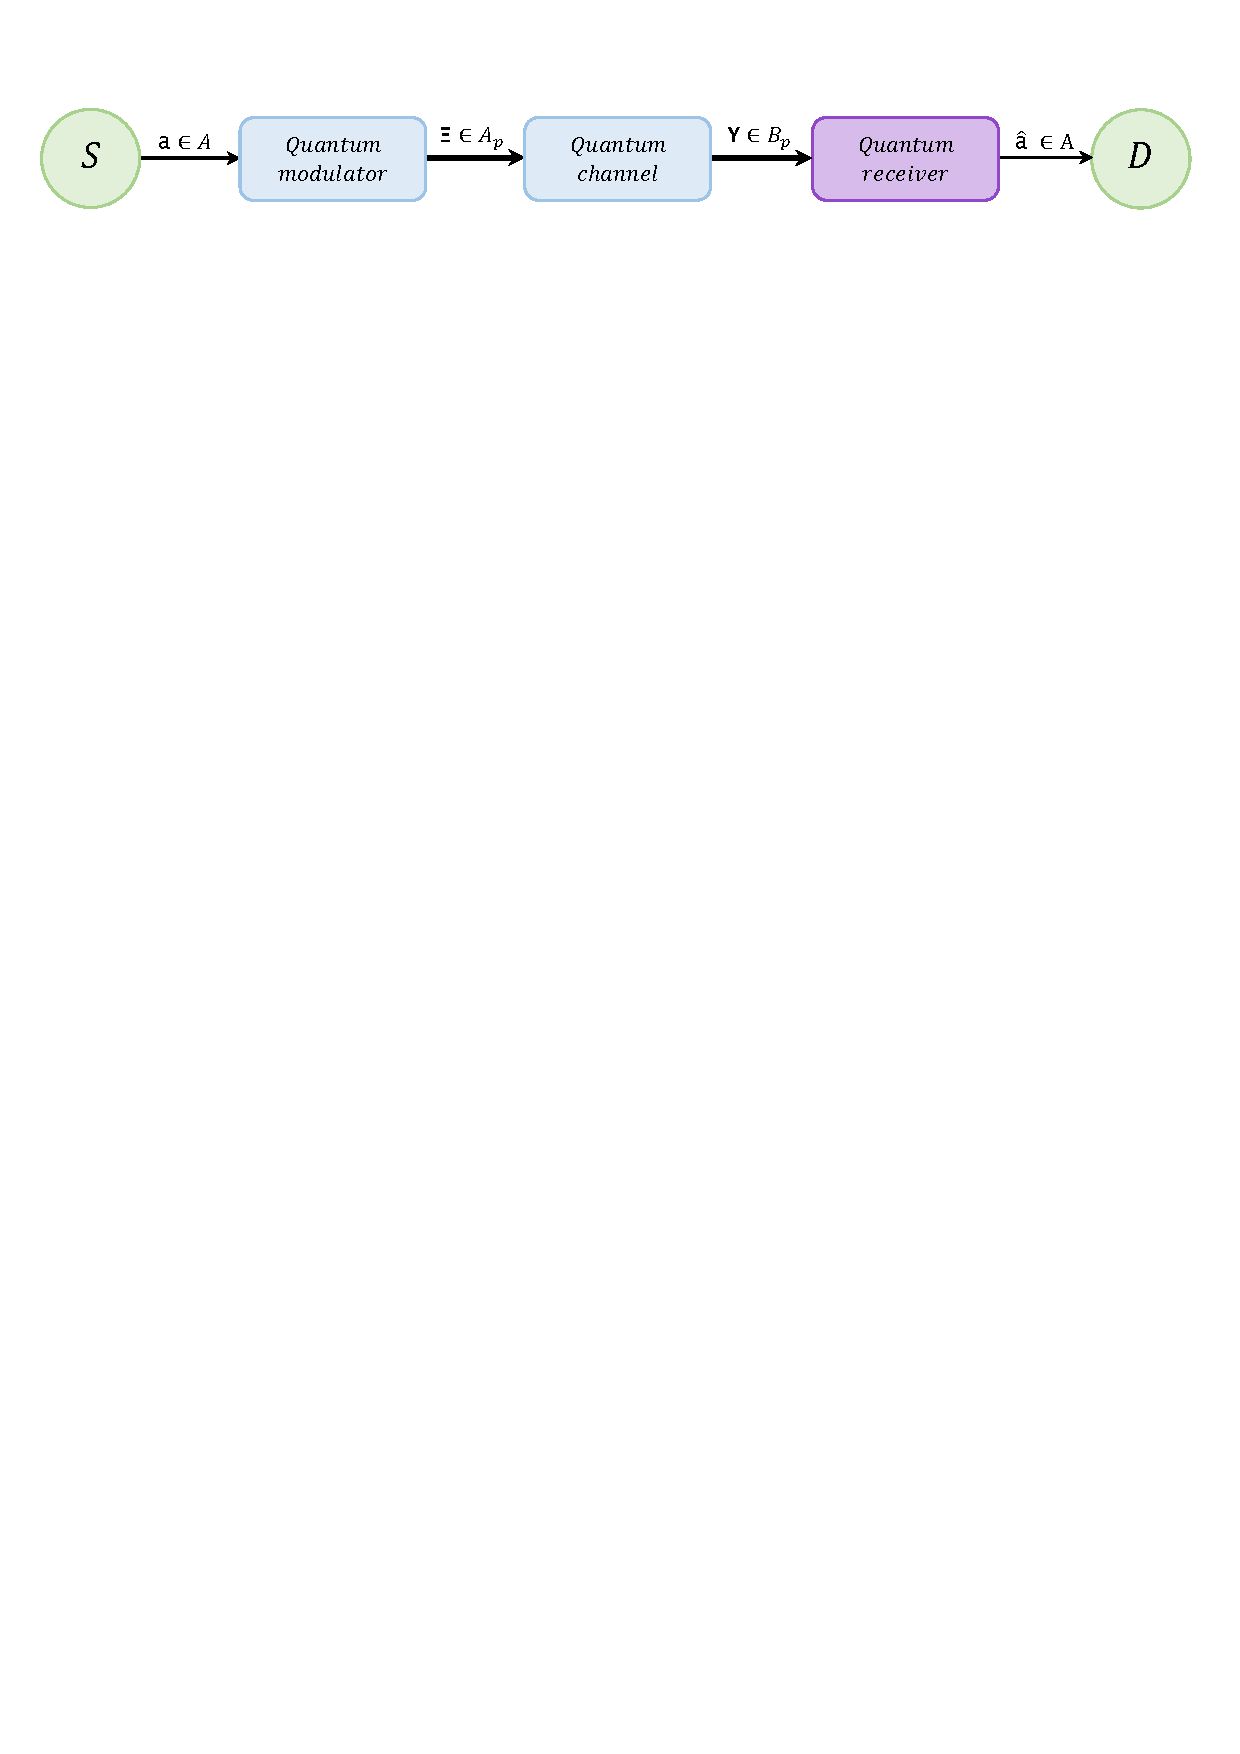
\includegraphics[width=1\textwidth]{Pictures/fig3.0.pdf}
    \begin{center}
        {\scriptsize 
        Block chain of a quantum communication system.
        }
    \end{center}
\end{frame}
    \subsection{Quantum modulator}
    \section{Quantum Modulation}
    As in a classical system, it is possible to define the concept of modulation for a 
    quantum communication system. The transmitted information will be associated to a 
    quantum state of the electromagnetic field, so it can be transmitted on the communication 
    channel.

    \begin{figure}[tbp]
        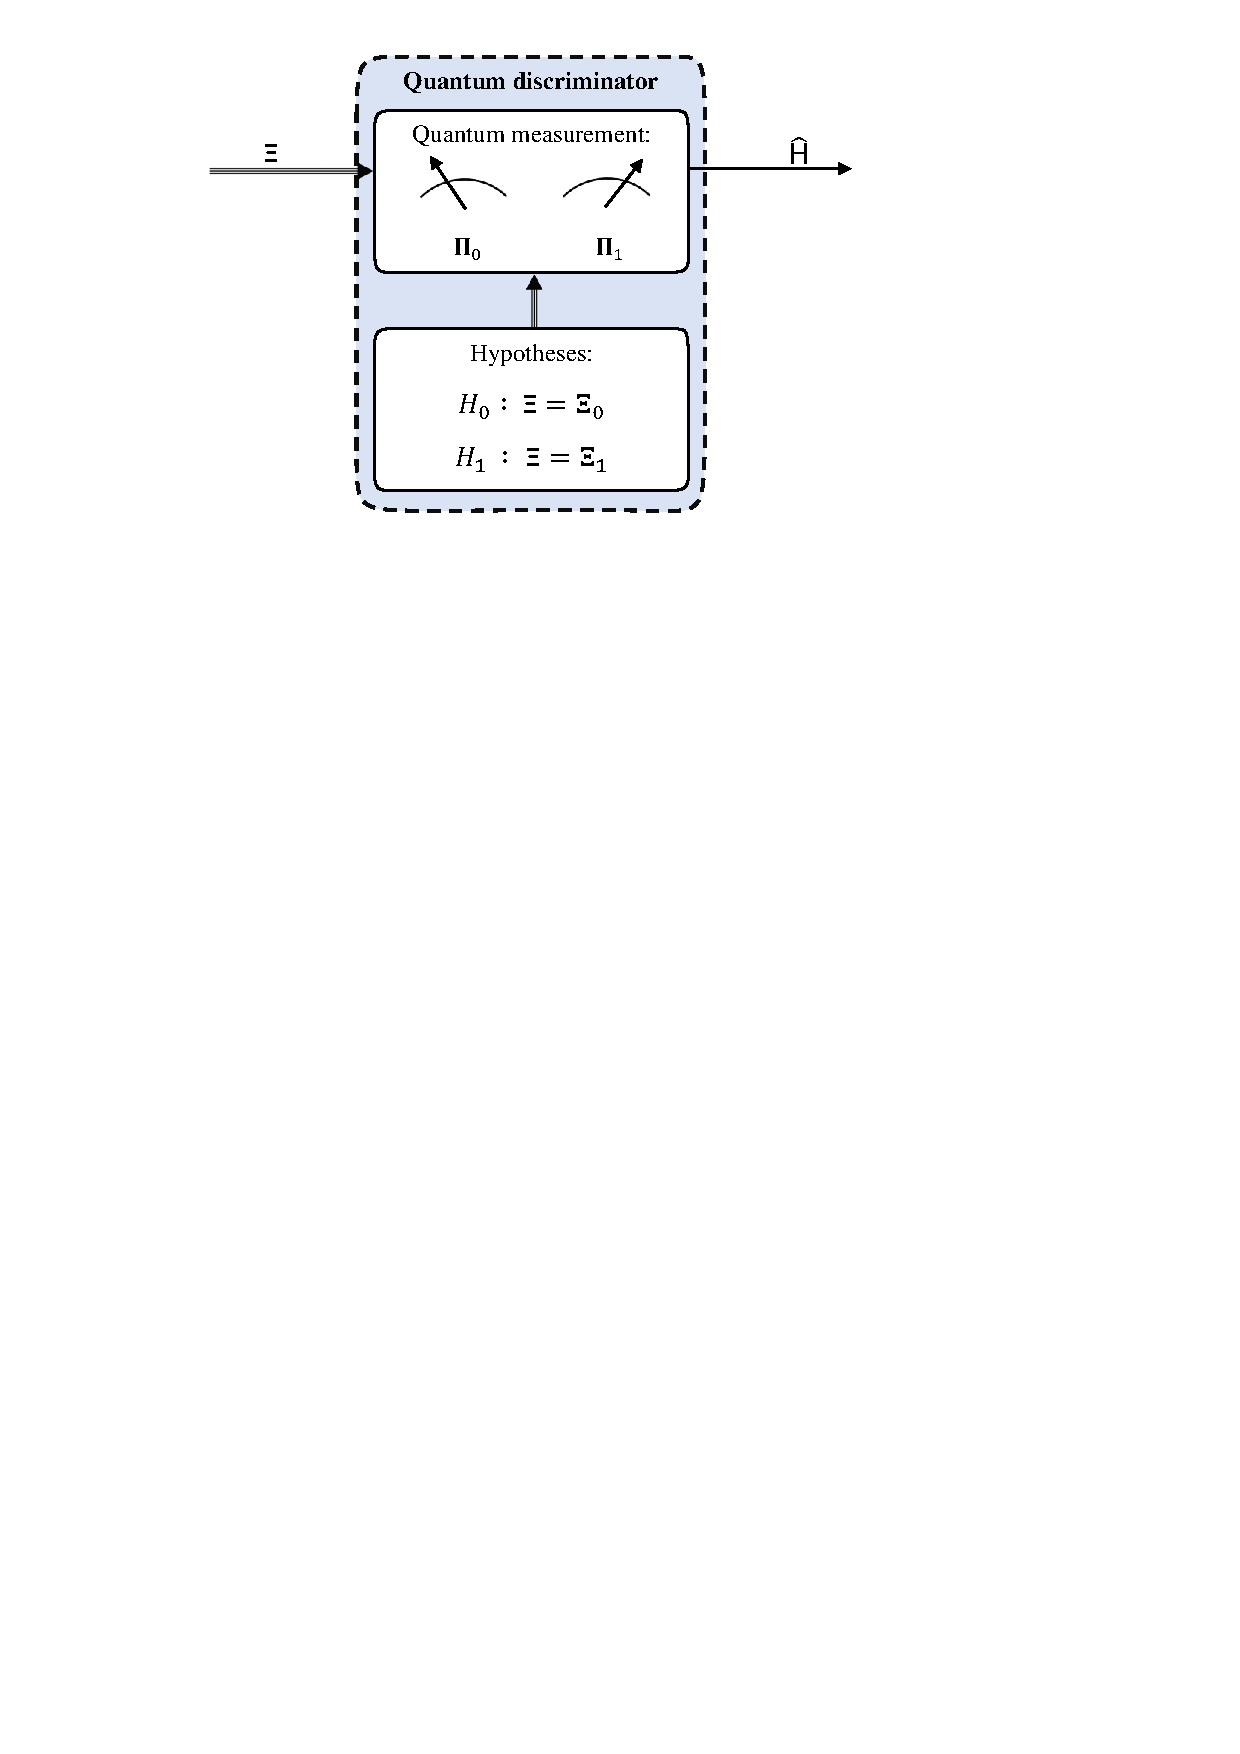
\includegraphics[width=1\textwidth]{fig2.1.pdf}
        \caption{Block diagram of a quantum transmitter.}
        \label{fig:2.1}
    \end{figure}
    It is possible to think about the quantum transmitter as in figure \ref{fig:2.1}. The bit source
    emits a bit sequence $a[n]$, the serial-parallel converter parallelizes a group of $l$-bit (where
    if $L$ is the number of quantum states, $l=\log_2(L)$) and sends them to the quantum modulator.
    This latter associates one quantum state to every group of bit. The operation of quantum state 
    creation, in real cases, is affected by noise.

    The sequence of operations is very close to a classical transmitter: the main difference is that
    the modulator maps the bits into quantum states instead of classical modulation. Therefore, it is 
    possible to achieve the quantum equivalent of classical modulation, with several states. After 
    that, the impact on performance can be tested.
    This thesis only considers and assesses the binary cases, in the OOK and BPSK 
    configuration.
    
    \subsection{OOK modulation}
        The OOK (on-off keying) is the most simple possible configuration for a communication system.
        The quantum implementation of that is realized associating the low-energy state to the 
        ground state $\ket{0}$ and the high-energy state to another state. It is important to
        consider that the physical realization of these states are not free-noise; this issue will be
        considered using noisy states \ref{eq:2.1.1}.
        \begin{equation}
            \pmb{\Xi}_0 = \pmb{\Xi}_{th}
            \label{eq:2.1.1}
        \end{equation}
        \begin{equation*}
            \pmb{\Xi}_1 = \pmb{\Xi}_{th}(\mu)
        \end{equation*}
        In the equation \ref{eq:2.1.1}, the high-energy state is associated to a coherent state. This 
        configuration has been widely analyzed in \cite{helstrom1,helstrom2,coherentComm1,coherentComm2,
        coherentComm3,coherentComm4} but this is not the only possible way. The use of PACS states 
        $\pmb{\Xi}_{th}^{(k)}(\mu)$ is analyzed in \cite{PACSDisc,tesiGuerrini}; the use of PASS are briefly
        assessed in the following chapter of this thesis.

    \subsection{BPSK modulation}
        BPSK quantum systems are implemented using two states with opposite amplitude, like
        \begin{equation}
            \pmb{\Xi}_0 = \pmb{\Xi}_{th}(-\mu)
            \label{eq:2.1.2}
        \end{equation}
        \begin{equation*}
            \pmb{\Xi}_1 = \pmb{\Xi}_{th}(\mu).
        \end{equation*}
        There is no guarantee that the use of a BPSK solution in  a quantum system will 
        improve its performance. The effect depends on which are the used states. In the next chapter some 
        configuration are assessed.

    \begin{frame}{Quantum Communication System}{Some important states}
    \begin{columns}

        \begin{column}{0.5\textwidth}
            \center{\underline{Coherent state}}
            \begin{equation*}\begin{split}
                &\Operator{A}\ket{\mu}=\mu\ket{\mu}\\
                &\ket{\mu}=\Operator{D}_\mu\ket{0}
            \end{split}\end{equation*}
            \\ \mbox{}
            \center{\underline{Thermal noise state}}
            \begin{equation*}\begin{split}
                &\Operator{\varXi}_{\mathrm{th}}=(1-v)\sum_{n=0}^{\infty}v^n\ket{n}\bra{n}\\
                v=&\frac{\bar{n}}{\bar{n}+1};\ \ \ \ 
                \bar{n}=\left(\exp{\frac{\hbar\omega}{k_B T}}-1\right)^{-1}
            \end{split}\end{equation*}
        \end{column}
        \begin{column}{0.5\textwidth}
            \center{\underline{Squeezed state}}
            \begin{equation*}
                \ket*{\mu,\zeta}=\Operator{D}_\mu\Operator{S}_\zeta\ket{0}
            \end{equation*}
            \\ \mbox{}
            \center{\underline{Photon added states}}\\
            \begin{equation*}
                \Operator{\varXi}^{(k)}=\frac{(\Operator{A}^\dagger)^k\Operator{\varXi}\pmb{A}^k}
                {\tr{(\Operator{A}^\dagger)^k\Operator{\varXi}\Operator{A}^k}}
            \end{equation*}
            \mbox{}
            %\hspace*{30pt}
            \mbox{}
        \end{column}
    \end{columns}

    \ \\ \mbox{} \\ \ \mbox{}
\end{frame}
    \subsection{Quantum receiver}
    \section{Quantum Discriminator}
    The problem of quantum state discrimination (QSD) is one of the most important
    aspects of quantum communication. As in classical communication, the ability to 
    distinguish between two or more states in presence of noise can be decisive in order to determine
    the performance of the communication system. However, differently from the classical situation,
    the discrimination can be done using a custom-designed quantum discriminator, overcoming
    the classical physics limits.

    \subsection{Binary quantum state discrimination}
    \begin{figure}[ht]
        \begin{center}
            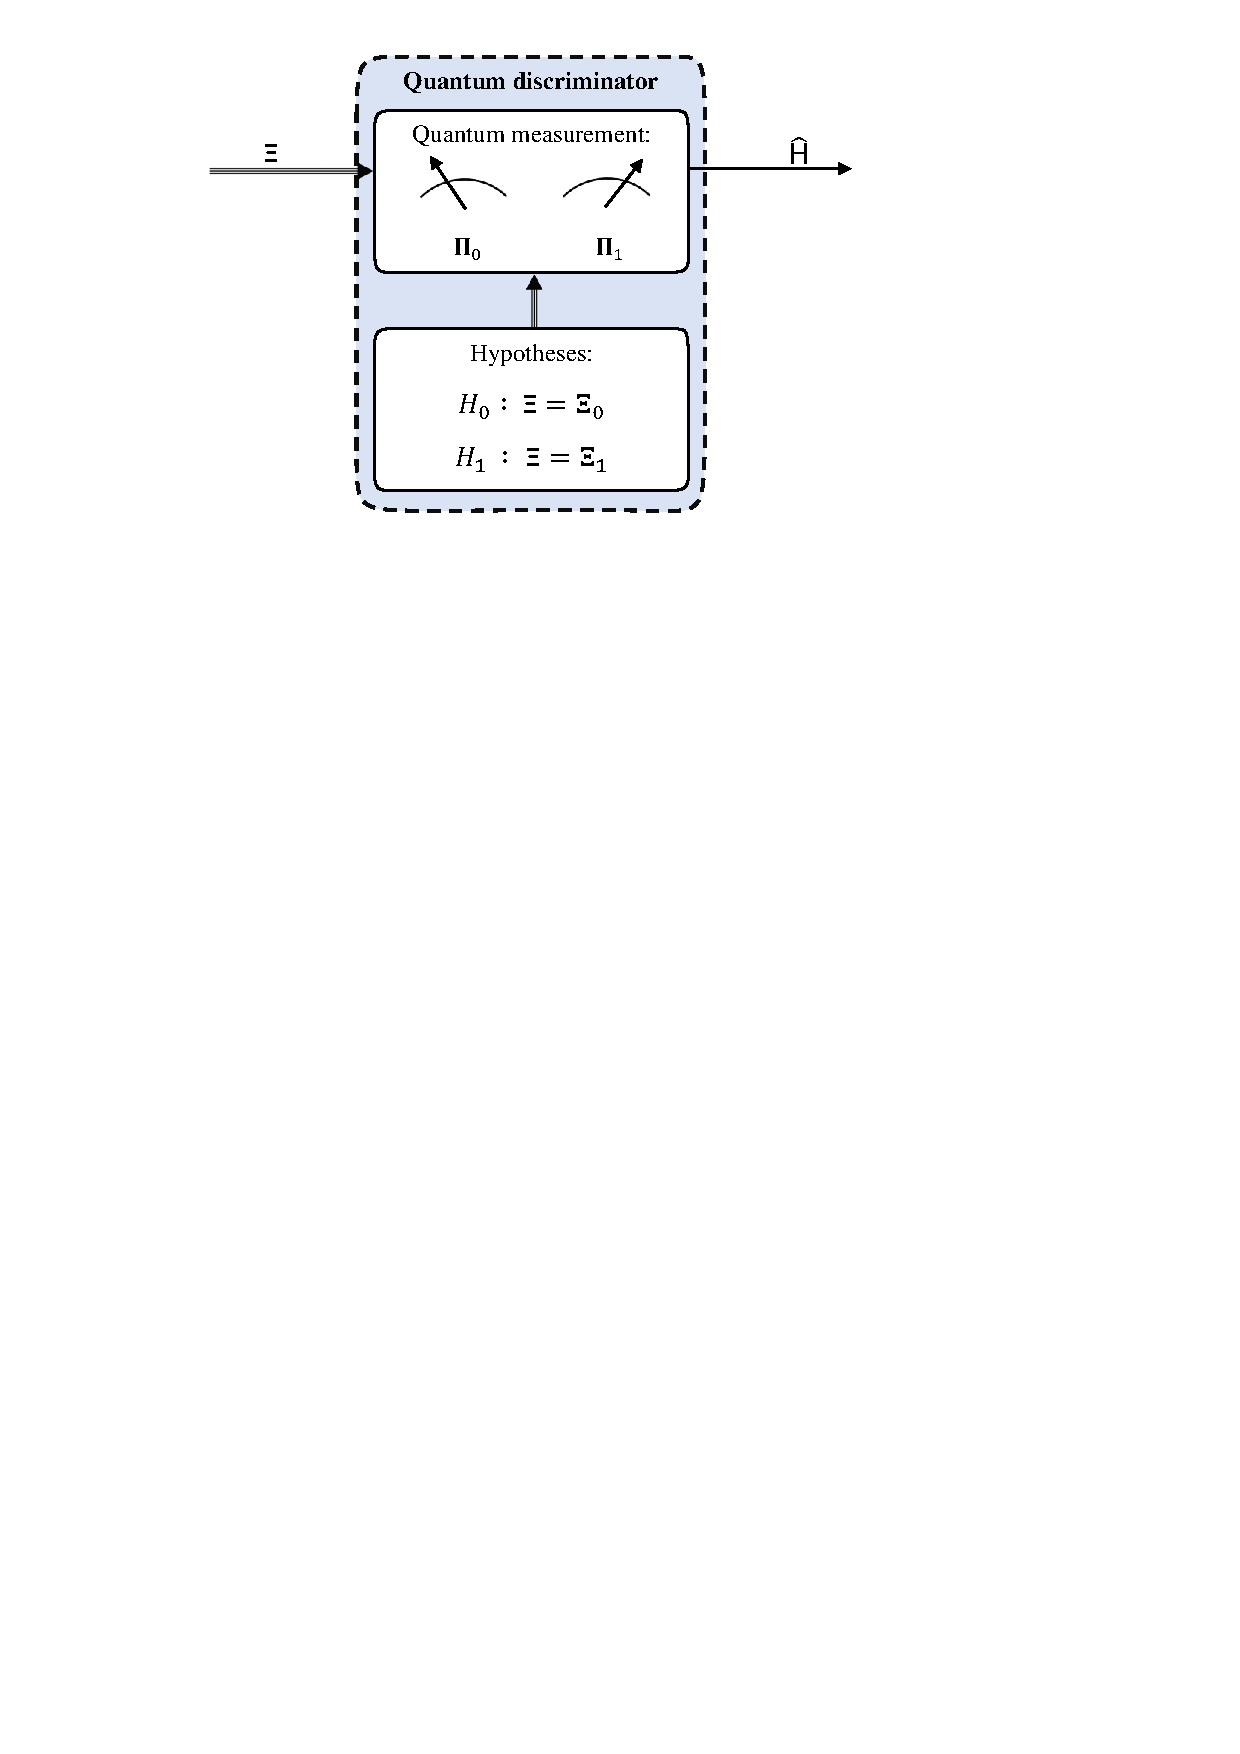
\includegraphics[width=0.75\textwidth]{fig2.2.pdf}
            \caption{Binary quantum state discriminator.}
            \label{fig:2.2}
        \end{center}
    \end{figure}
    The problem of discrimination between two quantum states is realized, as every measurement
    process \ref{post:2}, using an operator or a set of operators.
    If the state of the system is unknown, as shown in figure \ref{fig:2.2}, there are two hypotheses
    about the state $\pmb{\Xi}$ (the problem is easly generalizable for $M$ different states),
    given by:
    \begin{equation}\begin{split}
        H_0 : \pmb{\Xi}=\pmb{\Xi}_0\\
        H_1 : \pmb{\Xi}=\pmb{\Xi}_1
        \label{eq:binHyp}
    \end{split}\end{equation}
    It is necessary a set of two positive-definites operator (POVM)
    \begin{equation}
        \mathcal{P}=\{\pmb{\Pi}_0,\pmb{\Pi}_1\}
    \end{equation}
    for the discrimination process, and the probability that the hypothesis $H_j$ is choosen
    if $H_k$ is the right choose is given by \cite{tesiGuerrini}:
    \begin{equation}
        \mathbb{P}\{H_j|H_k\}=tr\{\pmb{\Xi}_k\pmb{\Pi}_j\}.
    \end{equation}
    The distribution error probability (DEP) in the discrimination process, if $p_0$ and $p_1$ are 
    respectively the probabilty of symbols $0$ and $1$, is so given by
    \begin{equation}
        P_e=1-\left(p_0 tr\{\pmb{\Xi}_0\pmb{\Pi}_0\}+p_1 tr\{\pmb{\Xi}_1\pmb{\Pi}_1\}\right).
    \end{equation}

    \subsection{Optimal discriminator}
    The issue of finding the optimal POVM that minimizes the DEP was exhaustively discuss  by Helstrom in 
    \cite{helstrom3,helstrom4}. The minimum distribution error probability (MDEP) for a binary 
    communication system is given by the well-known Helstrom bound
    \begin{equation}
        \breve{P}_e = \frac{1}{2} \left(1-\norm{p_1 \pmb{\Xi}_1 - p_0 \pmb{\Xi}_0}_1 \right),
        \label{eq:HelstromBound}
    \end{equation}
    where $p_0,\ p_1$ are the probability that the states $\pmb{\Xi}_0,\ \pmb{\Xi}_1$ are trasmitted
    and the operator $\norm{\cdot}_1$ represents the trace norm. 
    The MDEP \ref{eq:HelstromBound} is obtained with the following POVM:
    \begin{equation}
        \breve{\pmb{\Pi}}_0 = \sum_{\substack{i \\ \lambda_i<0}} \ket{\lambda_i}\bra{\lambda_i},
    \end{equation}
    \begin{equation*}
        \breve{\pmb{\Pi}}_1 = 1-\breve{\pmb{\Pi}}_0 = 
        \sum_{\substack{i \\ \lambda_i \geq 0}} \ket{\lambda_i}\bra{\lambda_i};
    \end{equation*}
    where $\ket{\lambda_i}$ is the eigenvector of $p_1 \pmb{\Xi}_1 - p_0 \pmb{\Xi}_0$ associated to 
    the eigenvalue $\lambda_i$.
    For pure states, i.e $\pmb{\Xi}_0 = \ket{\psi_0}\bra{\psi_0}$ and $\pmb{\Xi}_1 = \ket{\psi_1}
    \bra{\psi_1}$, the equation \ref{eq:HelstromBound} begin
    \begin{equation}
        \breve{P}_e = \frac{1}{2} \left(1- \sqrt{1-4 p_0 p_1 \absolutevalue{\braket{\psi_0}{\psi_1}}^2}
        \right).
        \label{eq:HelstromBPure}
    \end{equation}
    It is possible to observe that, for pure states, the MDEP is equal to $0$ if $\braket{\psi_0}{\psi_1}$,
    that is $\ket{\psi_0}$ and $\ket{\psi_1}$ are orthogonal states.

    % Capitolo 3: Discrimination of Photon Added States
    \section{Performance Analysys}
    \subsection{PACS system performance}
    %\begin{frame}{Discrimination of Photon Added States}{Noisy PACS discrimination: OOK}
%    \begin{center}
%        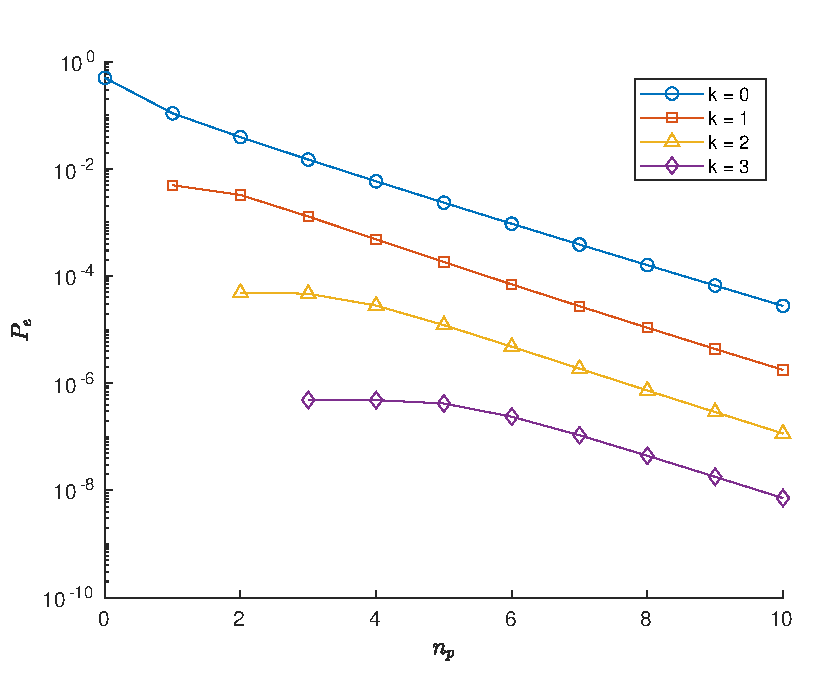
\includegraphics[width=0.65\textwidth]{Pictures/fig3.1.pdf}\\
%        \scriptsize{
%        MDEP of a QOOK system with PACS in terms of the mean photon number $n_p$.\\
%        $k=0,1,2,3$; $N=30$; $\bar{n}=10^{-2}$; $p_0=p_1=1/2$
%        }
%    \end{center}
%\end{frame}

\begin{frame}{Discrimination of Photon Added States}{Noisy PACS discrimination}
    \begin{center}
        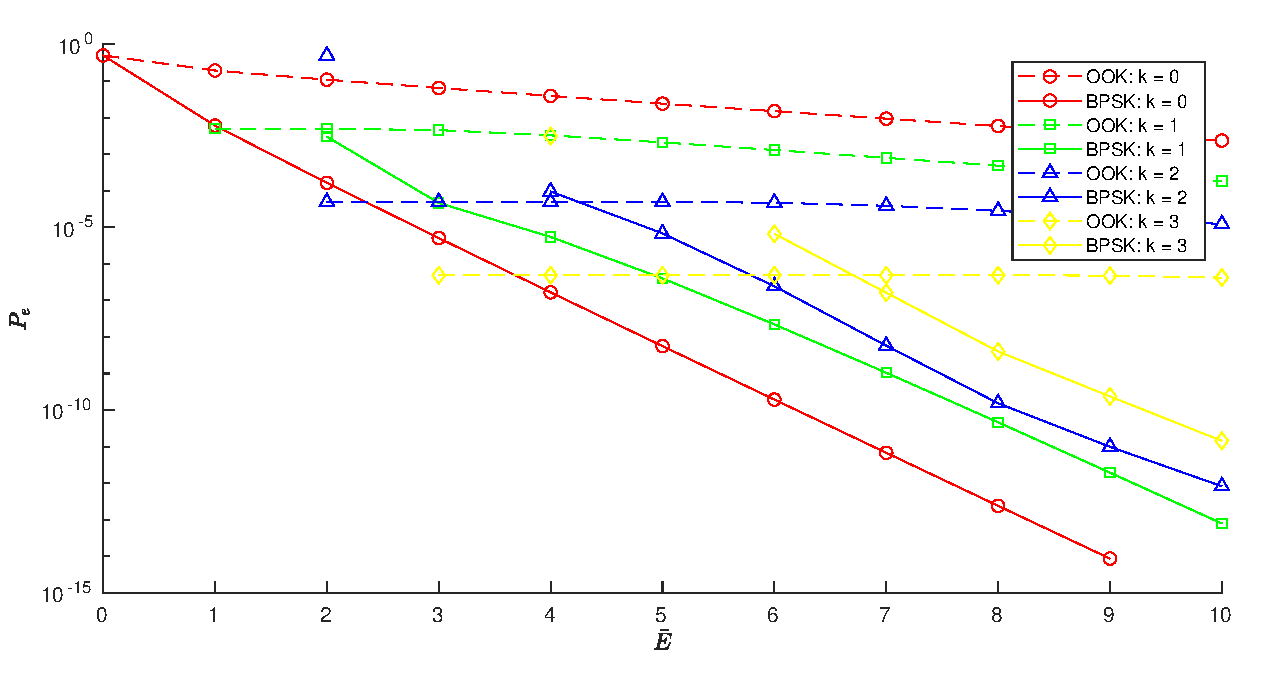
\includegraphics[width=0.9\textwidth]{Pictures/fig3.4.pdf}\\
        \scriptsize{
        MDEP comparison of a QOOK and QBPSK systems with PACS in terms of the mean energy of the system $\bar{E}$.\\
        $N=45$; $\bar{n}=10^{-2}$; $p_0=p_1=1/2$
        }
    \end{center}
    \ \mbox{}\\ \ \mbox{}\\
\end{frame}
    \subsection{Noise effect}
    \begin{frame}{Discrimination of Photon Added States}{Noise effect}
    \begin{columns}
        \begin{column}{0.5\linewidth}
            \begin{center}
                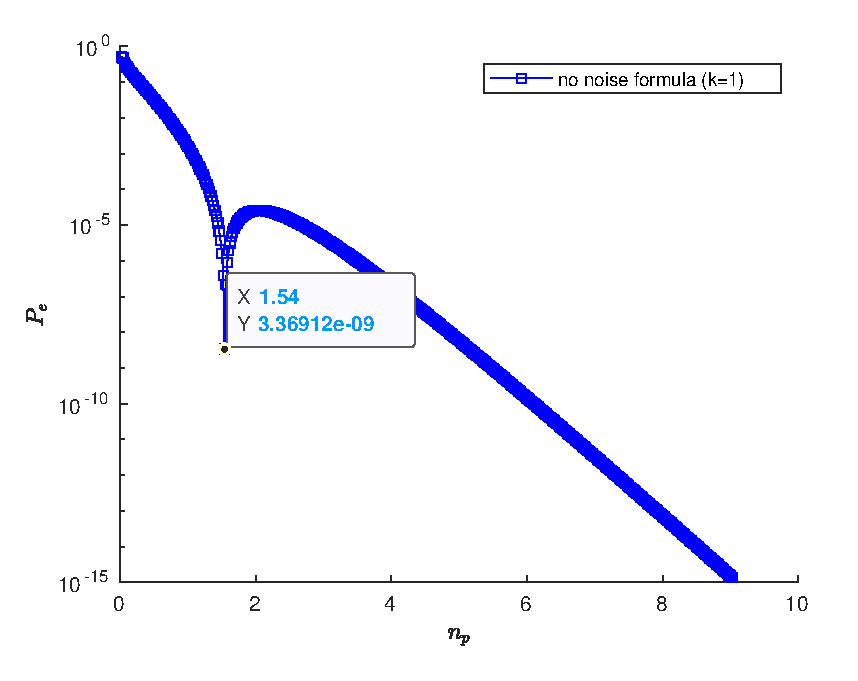
\includegraphics[width = 1\linewidth]{Pictures/fig3.2a.pdf}\\
                \scriptsize{
                    MDEP of a QBPSK with PACSs, without noise. $k=1$. 
                }
            \end{center}
        \end{column}
        \begin{column}{0.5\linewidth}
            \begin{center}
                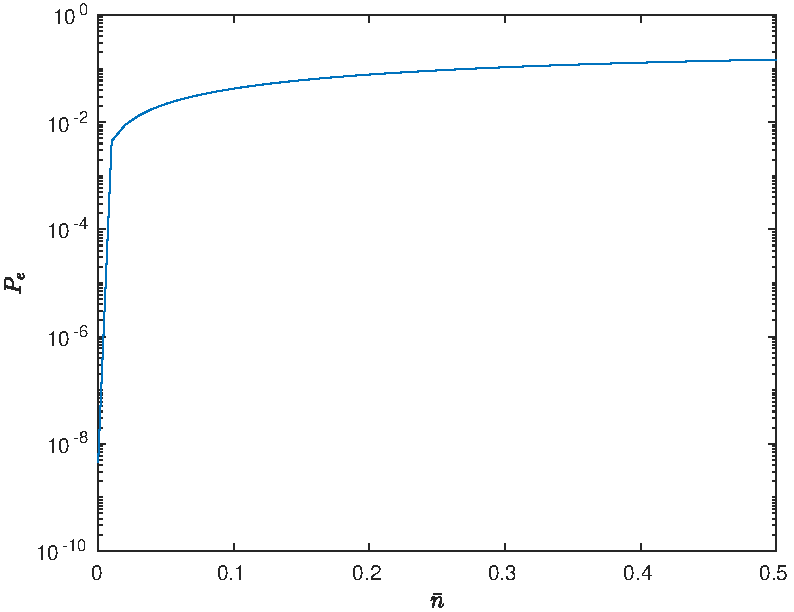
\includegraphics[width = 1\linewidth]{Pictures/fig3.3a.pdf}\\
                \scriptsize{
                    MDEP for $\mu=0.54$ (value of the zero) in terms of $\bar{n}$. 
                }
            \end{center}
        \end{column}
    \end{columns}
\end{frame}
    \subsection{Squeezed state system performance}
    \begin{frame}{Discrimination of Photon Added States}{Squeezed States discrimination: BPSK}
    \begin{center}
        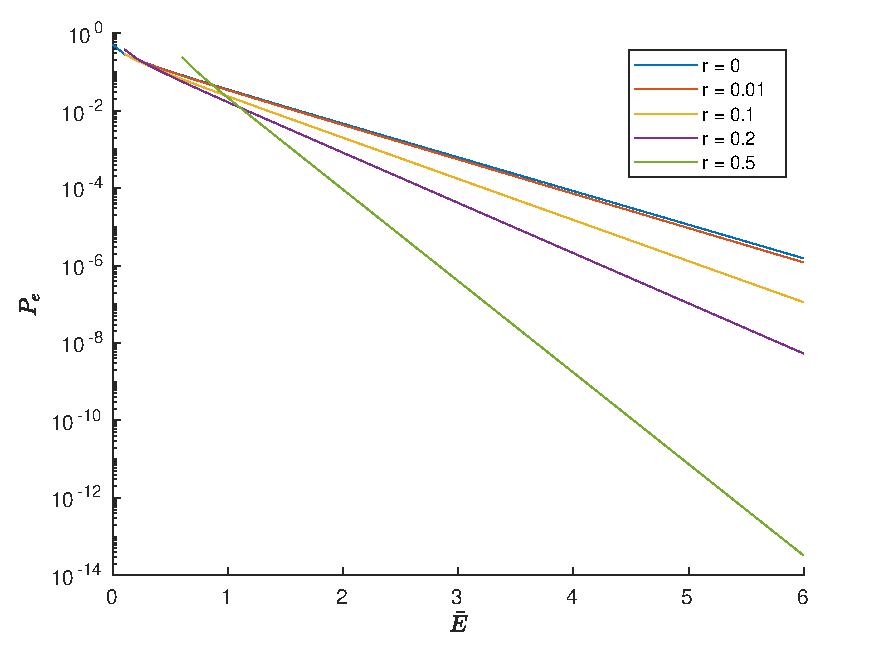
\includegraphics[width=0.67\textwidth]{Pictures/fig3.5.pdf}\\
        \scriptsize{
        MDEP of a QBPSK system with squeezed states in terms of the mean energy of the system $\bar{E}$.\\
        $N=30$; $\bar{n}=0$; $p_0=p_1=1/2$
        }
    \end{center}

\end{frame}
    \subsection{PASS system performance}
    \begin{frame}{Discrimination of Photon Added States}{Noisy PASS discrimination}
    \center{\scriptsize $N=45$; $\bar{n}=10^{-2}$; $\theta=\pi$; $p_0=p_1=1/2$}
    \begin{columns}
        \begin{column}{0.5\linewidth}%<1->
            \begin{center}
                \resizebox{1\textwidth}{!}{
                    % This file was created by matlab2tikz.
%
%The latest updates can be retrieved from
%  http://www.mathworks.com/matlabcentral/fileexchange/22022-matlab2tikz-matlab2tikz
%where you can also make suggestions and rate matlab2tikz.
%
\definecolor{mycolor1}{rgb}{0.00000,0.44706,0.74118}%
\definecolor{mycolor2}{rgb}{0.85098,0.32549,0.09804}%
\definecolor{mycolor3}{rgb}{0.92941,0.69020,0.12941}%
\definecolor{mycolor4}{rgb}{0.49020,0.18039,0.56078}%
\definecolor{mycolor5}{rgb}{0.46667,0.67451,0.18824}%
%
\begin{tikzpicture}

\begin{axis}[%
width=4.521in*0.75,
height=3.566in*0.75,
at={(0.758in,0.481in)},
scale only axis,
xmin=0,
xmax=4,
xlabel style={font=\color{white!15!black}},
xlabel={$\bar{n}_p$},
ymode=log,
ymin=1e-07,
ymax=1,
yminorticks=true,
ylabel style={font=\color{white!15!black}},
ylabel={$\breve{P}_e$},
axis background/.style={fill=white},
%axis x line*=bottom,
%axis y line*=left,
legend style={at={(0.01,0.01)}, anchor=south west, legend cell align=left, align=left, draw=white!15!black, legend columns=2}
]
\addplot [color=mycolor1, dashed, line width=1.0pt, mark=o, mark options={solid, mycolor1}, mark repeat={4}]
  table[row sep=crcr]{%
%0.0100000000010203	0.5\\
0.0100000000005099	0.451090572691058\\
0.0250000000005101	0.402886691283792\\
0.0500000000005101	0.356065452094155\\
0.08500000000051	0.311248795396144\\
0.13000000000051	0.268980151318818\\
0.18500000000051	0.229705791588748\\
0.25000000000051	0.193761885698297\\
0.32500000000051	0.161367836859558\\
0.41000000000051	0.132626017381623\\
0.50500000000051	0.107527572164159\\
0.61000000000051	0.0859635483991091\\
0.72500000000051	0.0677402706067526\\
0.850000000000511	0.0525976380078704\\
0.98500000000051	0.0402288938163128\\
1.13000000000051	0.030300412747497\\
1.28500000000051	0.0224701735043473\\
1.45000000000051	0.0164038154402497\\
1.62500000000051	0.0117874985937506\\
1.81000000000051	0.00833715723539569\\
2.00500000000051	0.00580411358757593\\
2.21000000000051	0.00397735316445369\\
2.42500000000051	0.00268301603344667\\
2.65000000000051	0.00178180465531275\\
2.88500000000051	0.00116504474732931\\
3.13000000000051	0.000750076554437373\\
3.38500000000051	0.000475529564681665\\
3.65000000000051	0.000296878649024612\\
3.92500000000051	0.000182524960914532\\
};
\addlegendentry{$r = 0.0$, $k = 0$}

\addplot [color=mycolor1, line width=1.0pt, mark=o, mark options={solid, mycolor1}, mark repeat={4}]
  table[row sep=crcr]{%
%1.02000000000307	0.00495049504950945\\
0.519950970393687	0.00495049504951145\\
0.549238056382468	0.00495049384760837\\
0.596318098365133	0.00494513949975245\\
0.659059689574124	0.00485212464085472\\
0.735198210318913	0.00459825907392819\\
0.822700461899245	0.00420399327465371\\
0.919966333468088	0.00369559902026673\\
1.02587839224384	0.00312976798911424\\
1.13975229329811	0.00256690084404709\\
1.26124327363325	0.00204996332234814\\
1.39024719180321	0.00160098998755381\\
1.52681572702182	0.00122639811266967\\
1.67109195414956	0.000923250889520943\\
1.8232653201361	0.000683888328226578\\
1.98354224079897	0.000498830625317581\\
2.15212812011347	0.000358440774981539\\
2.32921719287323	0.000253800056086939\\
2.51498745769556	0.000177110101371558\\
2.70959877008803	0.000121819045365512\\
2.91319279840464	8.25922216302066e-05\\
3.1258940040236	5.52004961243968e-05\\
3.34781112191599	3.63708050424849e-05\\
3.57903882606496	2.36261622261202e-05\\
3.81965939805169	1.51315705133603e-05\\
};
\addlegendentry{$r = 0.0$, $k = 1$}

\addplot [color=mycolor2, dashed, line width=1.0pt, mark=square, mark options={solid, mycolor2}, mark repeat={4}]
  table[row sep=crcr]{%
%0.0202340453657284	0.464473627654879\\
0.0151170226828645	0.437604627349995\\
0.0301170226828643	0.392232608937378\\
0.0551170226828643	0.345350311735397\\
0.0901170226828644	0.299872457829165\\
0.135117022682864	0.256926510392587\\
0.190117022682864	0.217172327050335\\
0.255117022682864	0.181031813929761\\
0.330117022682864	0.148752335319914\\
0.415117022682864	0.120429087835948\\
0.510117022682864	0.0960200366887284\\
0.615117022682864	0.0753645347394633\\
0.730117022682865	0.0582063945825236\\
0.855117022682864	0.0442194749392917\\
0.990117022682864	0.033033747624904\\
1.13511702268286	0.0242600166699049\\
1.29011702268286	0.0175117313604393\\
1.45511702268286	0.012422724228866\\
1.63011702268287	0.0086601979591992\\
1.81511702268287	0.00593281764231124\\
2.01011702268286	0.00399425837705447\\
2.21511702268287	0.00264294241797458\\
2.43011702268287	0.00171892901031734\\
2.65511702268286	0.00109898195775715\\
2.89011702268287	0.000690756906602363\\
3.13511702268287	0.000426868293537996\\
3.39011702268287	0.000259369510946184\\
3.65511702268287	0.000154957633989594\\
3.93011702268287	9.10290546821124e-05\\
};
\addlegendentry{$r = 0.1$, $k = 0$}

\addplot [color=mycolor2, line width=1.0pt, mark=square, mark options={solid, mycolor2}, mark repeat={4}]
  table[row sep=crcr]{%
%1.05080244685835	0.00494855515487186\\
0.534305855441027	0.00493956193944328\\
0.560577815242343	0.00489125057574918\\
0.603010711176586	0.00476554057726364\\
0.659935286045382	0.00454063398198279\\
0.729573342297954	0.00420193412015313\\
0.810323033235768	0.00375582941028574\\
0.90091844851316	0.0032368659457353\\
1.00047082343265	0.00269516501446371\\
1.10843171757119	0.00217671120450486\\
1.22452096613732	0.00171213398444298\\
1.3486495574248	0.00131595523776701\\
1.4808530565899	0.00099074984674008\\
1.62124071752346	0.000731856527585784\\
1.76995971625628	0.000531006006724011\\
1.92717165481784	0.000378693077575321\\
2.09303809416422	0.000265572059704344\\
2.26771230591607	0.000183193116200464\\
2.45133509281032	0.000124323441114904\\
2.64403315014596	8.30191324586171e-05\\
2.8459189361002	5.45554227568412e-05\\
3.05709138017673	3.5284096614796e-05\\
3.27763700858953	2.24616790437393e-05\\
3.50763123129931	1.40753992720621e-05\\
3.74713964255157	8.68275836485299e-06\\
3.99621925419453	5.27284023565944e-06\\
};
\addlegendentry{$r = 0.1$, $k = 1$}

\addplot [color=mycolor3, dashed, line width=1.0pt, mark=triangle, mark options={solid, mycolor3}, mark repeat={4}]
  table[row sep=crcr]{%
%0.051346909637612	0.429393647208632\\
0.0306734548188061	0.411688903318411\\
0.045673454818806	0.373223243143298\\
0.070673454818806	0.329064496412081\\
0.105673454818806	0.284699966244283\\
0.150673454818806	0.242312311121901\\
0.205673454818806	0.20300894013495\\
0.270673454818806	0.167412745153845\\
0.345673454818806	0.135848539010154\\
0.430673454818806	0.108424113178776\\
0.525673454818806	0.085074901679797\\
0.630673454818806	0.0655975019569672\\
0.745673454818806	0.0496824127447445\\
0.870673454818806	0.0369476450892914\\
1.00567345481881	0.0269714468453113\\
1.15067345481881	0.0193219002119312\\
1.30567345481881	0.0135816008581836\\
1.47067345481881	0.00936630014651907\\
1.64567345481881	0.00633712474233589\\
1.83067345481881	0.00420668870569196\\
2.02567345481881	0.00273998478983489\\
2.23067345481881	0.00175130670345874\\
2.44567345481881	0.00109858125431284\\
2.67067345481881	0.000676400651179798\\
2.90567345481881	0.000408804118392059\\
3.15067345481881	0.000242545209768685\\
3.40567345481881	0.000141270680246663\\
3.67067345481881	8.07790992743973e-05\\
3.94567345481881	4.53451833415941e-05\\
};
\addlegendentry{$r = 0.2$, $k = 0$}

\addplot [color=mycolor3, line width=1.0pt, mark=triangle, mark options={solid, mycolor3}, mark repeat={4}]
  table[row sep=crcr]{%
%1.14443400452204	0.00479106599394818\\
0.579999501304023	0.00475077465542328\\
0.603041046327231	0.00463108156969505\\
0.640504199710634	0.00442827805532442\\
0.691224117225214	0.00413258381262105\\
0.753950466998375	0.00374355433932783\\
0.827545812383434	0.00327986823785392\\
0.911100241882687	0.00277718849843345\\
1.00396497754985	0.00227642511237597\\
1.10573089526536	0.0018115455221398\\
1.21618079241689	0.00140378131439783\\
1.33523645804668	0.0010619876604348\\
1.46291195118471	0.000785891546957074\\
1.5992772335824	0.000569691758631641\\
1.7444321745409	0.000404922413376918\\
1.89848917670023	0.000282385374672289\\
2.06156226583414	0.0001933054291125\\
2.23376070757581	0.000129931168492581\\
2.41518563437222	8.57733261649951e-05\\
2.60592858523409	5.56215786678416e-05\\
2.80607120496685	3.54369671975441e-05\\
3.01568560586141	2.21846003883308e-05\\
3.23483507482365	1.36482495925461e-05\\
3.46357493039391	8.25216498795411e-06\\
3.70195341365423	4.90393868035621e-06\\
3.9500125478046	2.86426889811731e-06\\
};
\addlegendentry{$r = 0.2$, $k = 1$}

\addplot [color=mycolor4, dashed, line width=1.0pt, mark=diamond, mark options={solid, mycolor4}, mark repeat={4}]
  table[row sep=crcr]{%
%0.286971123755774	0.330768077356153\\
0.148485561877887	0.321870897864741\\
0.163485561877887	0.2980861532608\\
0.188485561877887	0.265400945113278\\
0.223485561877887	0.229097440353421\\
0.268485561877887	0.192694408147652\\
0.323485561877887	0.158325364694675\\
0.388485561877887	0.127217381024676\\
0.463485561877887	0.0999991591056063\\
0.548485561877887	0.0768883603237902\\
0.643485561877887	0.0578110254090491\\
0.748485561877886	0.042489385074143\\
0.863485561877887	0.0305142243008485\\
0.988485561877887	0.0214056829491879\\
1.12348556187789	0.0146637973864988\\
1.26848556187789	0.0098079816862493\\
1.42348556187789	0.00640463929230534\\
1.58848556187789	0.00408314565752849\\
1.76348556187788	0.00254163692367282\\
1.94848556187788	0.00154491239086835\\
2.14348556187788	0.000917124936882341\\
2.34848556187788	0.000531801834133649\\
2.56348556187788	0.000301247165333363\\
2.78848556187787	0.000166721564607453\\
3.02348556187786	9.01545309603957e-05\\
3.26848556187785	4.76353769972571e-05\\
3.52348556187783	2.45938563666614e-05\\
3.78848556187779	1.24073309797912e-05\\
};
\addlegendentry{$r = 0.5$, $k = 0$}

\addplot [color=mycolor4, line width=1.0pt, mark=diamond, mark options={solid, mycolor4}, mark repeat={4}]
  table[row sep=crcr]{%
%1.85306548733767	0.00353641115520514\\
0.930796962701587	0.00348196426464287\\
0.943656157582369	0.00332231969133245\\
0.965295445105895	0.00306951882024781\\
0.995980641808412	0.00274452597887531\\
1.03601054788413	0.00237451347003192\\
1.08567365297189	0.0019883961081173\\
1.14521827738196	0.00161265536534688\\
1.21483826418498	0.00126811447852393\\
1.29467137765998	0.000968122366654389\\
1.38480564628563	0.000718538771233457\\
1.48528924260403	0.000519112688197765\\
1.59614083486364	0.000365447596944291\\
1.71735873922715	0.000250906556350627\\
1.84892823171401	0.000168117888699859\\
1.9908269892895	0.000109991365809137\\
2.14302891711736	7.02953013373975e-05\\
2.30550670737067	4.38998630067355e-05\\
2.47823346100084	2.67972348785284e-05\\
2.66118364860192	1.59921449159883e-05\\
2.85433362280369	9.33241343792357e-06\\
3.05766183728397	5.32614461246084e-06\\
3.27114888140597	2.97307164354166e-06\\
3.49477740479924	1.62328253511257e-06\\
3.7285319812022	8.66931754384126e-07\\
3.97239894341011	4.5286496330732e-07\\
};
\addlegendentry{$r = 0.5$, $k = 1$}
\end{axis}
\end{tikzpicture}%
                }\\
                \scriptsize{
                MDEP of a QOOK system with PASS in terms of the mean photon number in the system $\bar{n}_p$.\\
                }
            \end{center}
        %\end{frame}
        \end{column}
        
        \begin{column}{0.5\linewidth}%<2->
            %\begin{frame}{Discrimination of Photon Added States}{Noisy PASS discrimination: BPSK}
            \begin{center}
                \resizebox{1\textwidth}{!}{
                    % This file was created by matlab2tikz.
%
%The latest updates can be retrieved from
%  http://www.mathworks.com/matlabcentral/fileexchange/22022-matlab2tikz-matlab2tikz
%where you can also make suggestions and rate matlab2tikz.
%
\definecolor{mycolor1}{rgb}{0.00000,0.44706,0.74118}%
\definecolor{mycolor2}{rgb}{0.85098,0.32549,0.09804}%
\definecolor{mycolor3}{rgb}{0.92941,0.69020,0.12941}%
\definecolor{mycolor4}{rgb}{0.49020,0.18039,0.56078}%
\definecolor{mycolor5}{rgb}{0.46667,0.67451,0.18824}%
%
\begin{tikzpicture}

\begin{axis}[%
width=4.521in*0.75,
height=3.566in*0.75,
at={(0.758in,0.481in)},
scale only axis,
xmin=0,
xmax=10,
xlabel style={font=\color{white!15!black}},
xlabel={$\bar{n}_p$},
ymode=log,
ymin=1.11022302462516e-16,
ymax=1,
yminorticks=true,
ylabel style={font=\color{white!15!black}},
ylabel={$\breve{P}_e$},
axis background/.style={fill=white},
%axis x line*=bottom,
%axis y line*=left,
legend style={at={(0.01,0.01)}, anchor=south west, legend cell align=left, align=left, draw=white!15!black, legend columns=2}
]
\addplot [color=mycolor1, dashed, line width=1.0pt, mark=o, mark options={solid, mycolor1}, mark repeat={4}]
  table[row sep=crcr]{%
0.0200000000020406	0.5\\
0.0400000000020402	0.402886691283791\\
0.10000000000204	0.311248795396143\\
0.20000000000204	0.229705791588748\\
0.34000000000204	0.161367836859558\\
0.52000000000204	0.107527572164159\\
0.740000000002041	0.0677402706067528\\
1.00000000000204	0.040228893816313\\
1.30000000000204	0.0224701735043469\\
1.64000000000204	0.0117874985937501\\
2.02000000000204	0.00580411358757571\\
2.44000000000204	0.00268301603344689\\
2.90000000000204	0.00116504474732904\\
3.40000000000204	0.000475529564681332\\
3.94000000000204	0.00018252496091431\\
4.52000000000204	6.58942320924671e-05\\
5.14000000000204	2.2372962739603e-05\\
5.80000000000205	7.14262612222516e-06\\
6.50000000000204	2.14348977123358e-06\\
7.24000000000202	6.04459258424228e-07\\
8.02000000000186	1.60120172343348e-07\\
8.84000000000037	3.98308174776041e-08\\
9.69999999998796	9.30169952173543e-09\\
};
\addlegendentry{$r = 0.0$, $k = 0$}

\addplot [color=mycolor1, line width=1.0pt, mark=o, mark options={solid, mycolor1}, mark repeat={4}]
  table[row sep=crcr]{%
2.04000000000614	0.5\\
2.07980388157475	0.365238945696499\\
2.19695222552987	0.245075031520992\\
2.38527239346053	0.149666545304717\\
2.6362387582965	0.0824178394910576\\
2.94079284127565	0.0405450261122263\\
3.29080184759698	0.0176651515033895\\
3.67986533387235	0.0067767120762533\\
4.10351356897534	0.00229560228979309\\
4.55900917319244	0.000707434570884347\\
5.04497309453299	0.00021948919726017\\
5.56098876721283	8.28582489130203e-05\\
6.10726290808727	4.1022391904566e-05\\
6.68436781659824	2.27142595118912e-05\\
7.29306128054439	1.21004232845334e-05\\
7.93416896319587	5.8707409222869e-06\\
8.60851248045389	2.56977332785402e-06\\
9.31686877149291	1.01844033345566e-06\\
};
\addlegendentry{$r = 0.0$, $k = 1$}

\addplot [color=mycolor2, dashed, line width=1.0pt, mark=square, mark options={solid, mycolor2}, mark repeat={4}]
  table[row sep=crcr]{%
0.0404680907314567	0.5\\
0.0604680907314585	0.392901670542549\\
0.120468090731458	0.293128630573881\\
0.220468090731458	0.206620339442921\\
0.360468090731457	0.136941029534563\\
0.540468090731457	0.084941538631533\\
0.760468090731459	0.0491016108355734\\
1.02046809073146	0.026360899632598\\
1.32046809073146	0.0131130551179189\\
1.66046809073146	0.00603787611242568\\
2.04046809073146	0.00257369694341059\\
2.46046809073146	0.00101640450241469\\
2.92046809073146	0.000372205972558992\\
3.42046809073146	0.00012645461779881\\
3.96046809073146	3.98629468535416e-05\\
4.54046809073146	1.16575616797565e-05\\
5.16046809073146	3.16151968782208e-06\\
5.82046809073146	7.94771541634542e-07\\
6.52046809073146	1.85116668105501e-07\\
7.26046809073146	3.99314517562921e-08\\
8.04046809073146	7.97410959485489e-09\\
8.86046809073146	1.47367751335281e-09\\
9.72046809073146	2.51973775178271e-10\\
};
\addlegendentry{$r = 0.1$, $k = 0$}

\addplot [color=mycolor2, line width=1.0pt, mark=square, mark options={solid, mycolor2}, mark repeat={4}]
  table[row sep=crcr]{%
2.1016048937167	0.5\\
2.13722342176411	0.351557555027417\\
2.24231126096937	0.222160769918723\\
2.41204284470634	0.124222362453645\\
2.63974114418153	0.0603925042112791\\
2.91829336919182	0.0250484475022711\\
3.24129213294307	0.00872798119433771\\
3.60367379405264	0.00258598757293121\\
4.0018832937306	0.000741253402724129\\
4.43372687028477	0.000287093498001045\\
4.89808386454928	0.000162974574048513\\
5.39459822969919	9.8293093218349e-05\\
5.9234122263596	5.2962165794368e-05\\
6.48496287009384	2.48063685127087e-05\\
7.07983886502512	1.01844444848065e-05\\
7.70868661927138	3.70885692668743e-06\\
8.37215237665687	1.20946493997742e-06\\
9.07084922366429	3.55623495429391e-07\\
9.80534037124127	9.47534976036835e-08\\
};
\addlegendentry{$r = 0.1$, $k = 1$}

\addplot [color=mycolor3, dashed, line width=1.0pt, mark=triangle, mark options={solid, mycolor3}, mark repeat={4}]
  table[row sep=crcr]{%
0.102693819275224	0.5\\
0.122693819275224	0.381945077116474\\
0.182693819275225	0.273671210068553\\
0.282693819275225	0.18272455257\\
0.422693819275225	0.112952560216816\\
0.602693819275226	0.0642502792905548\\
0.822693819275224	0.03345396094764\\
1.08269381927522	0.0158838250522541\\
1.38269381927522	0.00686368066298626\\
1.72269381927522	0.00269897231763505\\
2.10269381927523	0.000966736234112642\\
2.52269381927523	0.000315777240763426\\
2.98269381927522	9.41232533182568e-05\\
3.48269381927522	2.56024275193667e-05\\
4.02269381927522	6.35315675889814e-06\\
4.60269381927523	1.43743867431212e-06\\
5.22269381927523	2.96354467355098e-07\\
5.88269381927523	5.5640574203597e-08\\
6.58269381927523	9.50809414534959e-09\\
7.32269381927523	1.47814516182621e-09\\
8.10269381927523	2.08976613791378e-10\\
8.92269381927523	2.68594035901515e-11\\
9.78269381927522	3.13798986795177e-12\\
};
\addlegendentry{$r = 0.2$, $k = 0$}

\addplot [color=mycolor3, line width=1.0pt, mark=triangle, mark options={solid, mycolor3}, mark repeat={4}]
  table[row sep=crcr]{%
2.28886800904409	0.5\\
2.31999800521609	0.335903697984307\\
2.41216418530892	0.196933331036258\\
2.56201679884254	0.0981076147304128\\
2.76489646890086	0.040185809256969\\
3.0158018679935	0.0130832203468926\\
3.31018324953374	0.00344887391962134\\
3.64440096753075	0.00101951363497232\\
4.01585991019939	0.000567040966715227\\
4.42292358106145	0.000392962039574174\\
4.86472316966757	0.000231481537813827\\
5.34094583218671	0.000111581978084918\\
5.85164780473884	4.51448958011524e-05\\
6.39710893432961	1.56946401249081e-05\\
6.97772869816361	4.76400489057838e-06\\
7.59395670680091	1.27574898745042e-06\\
8.24624906333657	3.03436716753147e-07\\
8.93504283030325	6.43988304904752e-08\\
9.66074253748888	1.2235391422255e-08\\
};
\addlegendentry{$r = 0.2$, $k = 1$}

\addplot [color=mycolor4, dashed, line width=1.0pt, mark=diamond, mark options={solid, mycolor4}, mark repeat={4}]
  table[row sep=crcr]{%
0.573942245572178	0.5\\
0.593942245028823	0.342499519674481\\
0.653942245170735	0.20790550335767\\
0.753942245341616	0.110057719920144\\
0.893942244583911	0.0500472584431716\\
1.07394224497389	0.0193143675146228\\
1.293942244546	0.00628332214973615\\
1.55394224371114	0.00172174882973891\\
1.85394224420503	0.000398395169961208\\
2.19394224278596	7.80046198984863e-05\\
2.57394224201761	1.29266966575337e-05\\
2.99394224220523	1.81130230003657e-06\\
3.45394223899107	2.14287482536157e-07\\
3.95394223844945	2.13728023612525e-08\\
4.49394223715584	1.79488168772224e-09\\
5.07394223021208	1.26788857190974e-10\\
5.693942230031	7.52714557350487e-12\\
6.35394222368679	3.74977826567147e-13\\
7.05394220748901	1.55431223447522e-14\\
7.79394220753813	4.44089209850063e-16\\
8.57394218450974	1.11022302462516e-16\\
9.39394214003978	0\\
};
\addlegendentry{$r = 0.5$, $k = 0$}

\addplot [color=mycolor4, line width=1.0pt, mark=diamond, mark options={solid, mycolor4}, mark repeat={4}]
  table[row sep=crcr]{%
3.7061308486222	0.5\\
3.72318775095693	0.276003723186423\\
3.77462452178882	0.111964236743116\\
3.86118165596315	0.0292098038693948\\
3.98392247081425	0.00541832505604978\\
4.14404207041508	0.00392337294658973\\
4.34269448841782	0.00386065139664005\\
4.58087300628471	0.00224591730584783\\
4.85935291484359	0.000870231139084243\\
5.17868537920139	0.000246879397142796\\
5.53922245734845	5.40728938508428e-05\\
5.94115678880561	9.42866109115981e-06\\
6.38456317979691	1.33219265713302e-06\\
6.86943477192184	1.54061789436888e-07\\
7.39571266351863	1.46675764867155e-08\\
7.96330772743687	1.15372272846415e-09\\
8.57211535637269	7.51390061282109e-11\\
9.22202638435226	4.05170341721828e-12\\
9.9129334474046	1.78523862359725e-13\\
};
\addlegendentry{$r = 0.5$, $k = 1$}
\end{axis}
\end{tikzpicture}%
                }\\
                \scriptsize{
                MDEP of a QBPSK system with PASS in terms of the mean photon number in the system $\bar{n}_p$.\\
                }
            \end{center}
        \end{column}
    \end{columns}
 \mbox{} \\ \mbox{} \\
\end{frame}  

    \section{Conclusion}
    % Conclusioni

\chapter{Conclusion}
    Questa tesi si pone come obiettivo di analizzare le prestazioni nella QSD (Quantum states discrimination) per 
    sistemi binari, in termini di probabilità di errore nel riconoscimento dei simboli, con l'utilizzo di un discriminatore ottimo.
    Sono stati presentati inizialmente i fondamenti della teoria meccanica quantistica nella formulazione di 
    Dirac-Neumann e nella sua generalizzazione tramite l'utilizzo di Density operator. Sono stati quindi descritti
    i concetti di modulazione quantum e di discriminazione di stati quantistici ed infine sono state analizzate le
    prestazioni di alcuni sistemi in termini di minimum distribution error probability (MDEP). 
    Tutte le valutazioni sono state fatte supponendo che la comunicazione non risenta di effetti associati al canale di comunicazione,
    dunque che lo stato emesso dal trasmettitore giunga al discriminatore del ricevitore senza modifiche.

    Questa tesi pone in evidenza come l'utilizzo di stati non Gaussiani (non-Gaussian states) photon added in sistemi OOK può 
    apportare un miglioramento nella QSD rispetto all'utilizzo di stati Gaussiani. La combinazione in particolare di squeezing 
    e photon addition (PASSs) risulta estremamante efficace.
    L'effetto della photon addition si manifesta invece negativo in sistemi quantistici BPSK.

    I risultati ottenuti possono essere di notevole importanza nel design di un sistema di comunicazione che sfrutti stati 
    quantistici, permettendo di sfruttare al meglio le potenzialità di questa teoria fisica.
\end{document}